% !TEX encoding = UTF-8
% !TEX TS-program = pdflatex
% !TEX root = ../../tesi.tex

\section{Il progetto}
Il progetto di stage, chiamato \textbf{NFTLab} e proposto dall'azienda Sync Lab, consiste in un \textit{e-commerce} dedicato alla vendita di NFT. Prima di spiegare le varie funzionalità e caratteristiche di NFTLab, è doveroso fare una premessa e spiegare cosa sono gli NFT. \\

\begin{figure}[!h]
  \centering
  
\includegraphics[width=0.1\columnwidth]{capitolo2/nft-logo.png}
  \caption{Simbolo degli NFT}
\end{figure}

Nati nel 2017 in seguito alla richiesta di standardizzazione su blockchain Ethereum ERC721, NFT è l'acronimo di \textit{Non Fungible Token} e per comprendere cosa sono e le loro possibili applicazioni, dobbiamo prima di tutto analizzare l'etimologia della parola.
Un \textit{token} lessicale è un'insieme di caratteri che rappresentano qualsiasi cosa e il fatto che sia non fungibile implica che rappresenta un qualcosa di unico.
In contrapposizione ai \textit{token} fungibili, come le monete fisiche o le \gls{criptovalute}, i \textit{token} non fungibili non possono essere scambiati reciprocamente in quanto ognuno ha un valore che non è legato al \textit{token} in sè, ma a quello che rappresenta.
Vengono salvati nella tecnologia \textit{blockchain} per semplificare la gestione dell'accesso e della proprietà e per assicurare l'unicità e l'impossibilità di contraffazione. \\

\noindent Gli NFT possono essere distinti dai token fungibili per le seguenti tre caratteristiche:
\begin{itemize}
  \item \textbf{Unico}: qualsiasi NFT viene definito da un codice univoco che lo rappresenta;
  \item \textbf{Raro}: questo è ciò che gli attribuisce il valore, in quanto se ce ne fossero di più varrebbero di meno;
  \item \textbf{Indivisibile}: gli NFT non possono essere suddivisi in parti, in quanto perderebbero il proprio valore. Devono essere detenuti, acquistati e venduti solo come entità intere.
\end{itemize}

\noindent Le applicazioni che possono avere sono di vario tipo, ma in generale possono essere utilizzati ovunque ci sia bisogno di questi tre benefici:
\begin{itemize}
  \item \textbf{Fornire la proprietà}: ovvero consolidare il diritto di proprietà, visto che ogni NFT deve essere associato ad una persona;
  \item \textbf{Trasferibilità}: i diritti di proprietà di un NFT possono essere negoziati su vari mercati e scambiati facilmente;
  \item \textbf{Dimostrare l'autenticità}: utilizzando la tecnologia \textit{blockchain} è possibile rassicurare i compratori dimostrando che il loro acquisto è autentico e originale.
\end{itemize}

L'ambito nel quale sono stati utilizzati sin da subito è l'arte digitale, dove c'è bisogno di dimostrare l'autenticità e la proprietà di una determinata opera per evitare contraffazioni.
Anche se esistono da tanti anni, si sono diffusi solo verso la fine del 2020 e inizio 2021 grazie a siti che permettono il caricamento e la vendita di opere digitali sotto forma di NFT. Il sito più famoso ed utilizzato in questo ambito si chiama \textit{CryptoKitties}, dove tutte le opere che si possono acquistare e vendere riguardano dei gatti, a cui ogni autore può applicare delle particolarità che rendono la sua opera unica.

\begin{figure}[!tbph]
  \captionsetup{singlelinecheck = false, format= hang, justification=raggedright, font=footnotesize, labelsep=space}

  \centering

  \begin{minipage}{0.5\textwidth}
    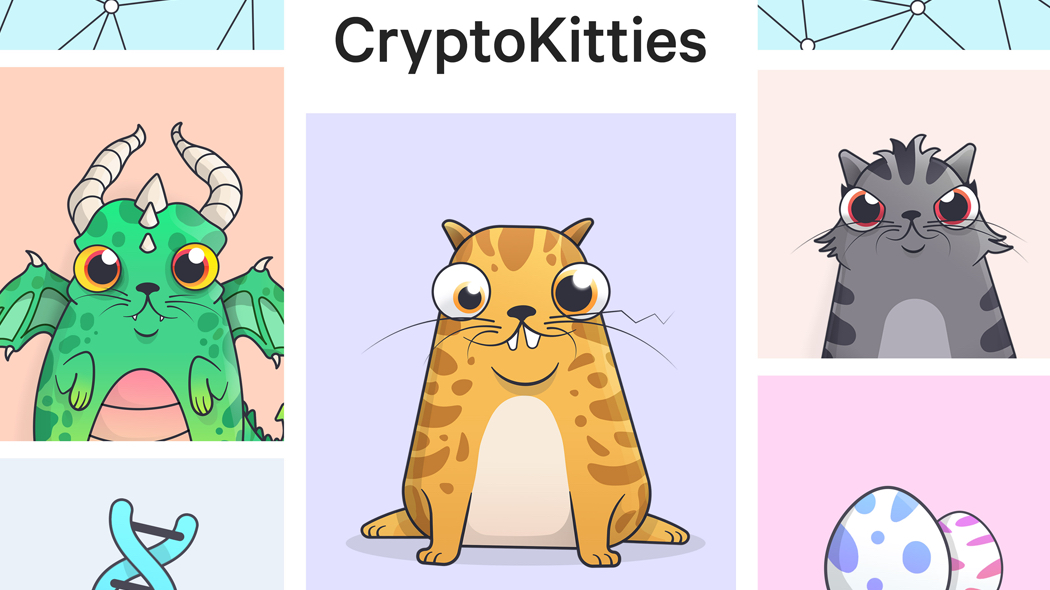
\includegraphics[width=\textwidth]{capitolo2/cryptokitties.jpg}
  \end{minipage}%
  \begin{minipage}{0.5\textwidth}
    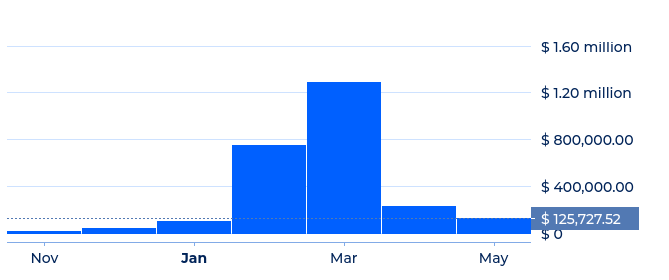
\includegraphics[width=\textwidth]{capitolo2/movimento-capitali-cryptokitties.png}
  \end{minipage}

  \begin{minipage}[t]{0.5\textwidth}
    \caption{Esempio di CryptoKitties}
    \textbf{Fonte}: \href{https://www.cryptokitties.co}{https://www.cryptokitties.co}
  \end{minipage}%
  \begin{minipage}[t]{0.5\textwidth}
    \caption{Movimento di capitali sulla piattaforma CryptoKitties, anno 2020/2021}
    \textbf{Fonte}: \href{https://coinranking.com/dapp/cryptokitties}{https://coinranking.com}
  \end{minipage}
\end{figure}

NFTLab è nato proprio da questo contesto. Oltre alle funzionalità di accesso e registrazione, permetterà agli utenti autenticati di caricare le proprie opere, che potranno essere qualsiasi tipo di \textit{file}, aggiungendo un nome, una descrizione, le categorie facente parte, il prezzo e gli verrà anche assegnato un tipo in base al \textit{file}. In seguito al caricamento verrà estratto il NFT e memorizzato in \textit{blockchain}. 
Ogni utente potrà visualizzare le opere caricate dalle altre persone, cercarle in base alle categorie di cui fanno parte, il loro tipo ed il nome, e comprarle, se autenticato. Quando visualizzerà i dettagli di un opera, in base al tipo del \textit{file}, verrà mostrata l'anteprima di quest'ultima.
I dati di ogni opera possono essere cambiati dal proprietario, tranne l'opera in sè visto che il NFT è intrinsecamente legato ad essa.

\begin{figure}[!h]
  \centering
  
\includegraphics[width=0.3\textwidth]{capitolo2/nftlab-logo.png}
  \caption{Logo di NFTLab}
\end{figure}

Il progetto è stato sviluppato con altre quattro persone che stavano svolgendo il percorso di stage dell'Università degli Studi di Padova. Due di queste persone avevano il compito di sviluppare il \textit{front-end} utilizzando, ognuna, un \textit{framework} tra Angular e Vue.js. La terza persona, invece, aveva il compito di sviluppare il \textit{back-end} attraverso il \textit{framework} Spring. La parte di creazione e gestione degli NFT l'ho fatta io. \\

\noindent In accordo con il proponente, al termine dello stage, sono state implementate le seguenti funzionalità:
\begin{itemize}
  \item registrazione ed autenticazione di un utente;
  \item caricamento di un opera ed inserimento delle relative informazioni;
  \item modifica di un'opera precedentemente caricata;
  \item visualizzazione della pagina personale di un utente;
  \item visualizzazione di tutte le opere caricate da altri utenti;
  \item visualizzazione dei dettagli di un opera.
\end{itemize}

\noindent Come già previsto dai nostri \textit{tutor} aziendali, tra cui il mio, Fabio Pallaro, in seguito all'arrivo di altri tirocinanti verranno ultimate le seguenti funzionalità:
\begin{itemize}
  \item vendita di un opera precedentemente caricata;
  \item ricerca di un opera precedentemente caricata.
\end{itemize}

Per quanto riguarda lo sviluppo della parte di gestione degli NFT, è stato pensato di progettare un percorso di stage dove un futuro tirocinante avrà il compito di sviluppare interamente una \gls{DApp}, rimuovendo la componente \textit{back-end} e affidando quel ruolo ad un singolo \textit{smart contract}.